\documentclass{article}
\title{CS 279 Assignment 2: Conduct an Experiment\\Part 1: Implementation}
\author{Miriam Cha and Melih Elibol}
\date{September 16, 2014}

\usepackage{amsmath}
\usepackage{bbm}
\usepackage{fullpage}
\usepackage{graphicx}
\usepackage{listings}
\usepackage[usenames,dvipsnames]{color}

\usepackage{amsmath,graphicx,amssymb,amsfonts,bbm,subfigure}
\usepackage{array,colortbl,xcolor}

\usepackage{tikz}
\usetikzlibrary{shapes,arrows}
\usepackage{caption}

%% This is the color used for MATLAB comments below
%\definecolor{MyDarkGreen}{rgb}{0.0,0.4,0.0}
%
%% For faster processing, load Matlab syntax for listings
%\lstloadlanguages{Matlab}%
%\lstset{language=Matlab,                        % Use MATLAB
%        frame=single,                           % Single frame around code
%        basicstyle=\small\ttfamily,             % Use small true type font
%        keywordstyle=[1]\color{Blue}\bf,        % MATLAB functions bold and blue
%        keywordstyle=[2]\color{Purple},         % MATLAB function arguments purple
%        keywordstyle=[3]\color{Blue}\underbar,  % User functions underlined and blue
%        identifierstyle=,                       % Nothing special about identifiers
%                                                % Comments small dark green courier
%        commentstyle=\usefont{T1}{pcr}{m}{sl}\color{MyDarkGreen}\small,
%        stringstyle=\color{Purple},             % Strings are purple
%        showstringspaces=false,                 % Don't put marks in string spaces
%        tabsize=4,                              % 4 spaces per tab
%        %
%        %%% Put standard MATLAB functions not included in the default
%        %%% language here
%        morekeywords={xlim,ylim,var,alpha,factorial,poissrnd,normpdf,normcdf},
%        %
%        %%% Put MATLAB function parameters here
%        morekeywords=[2]{on, off, interp},
%        %
%        %%% Put user defined functions here
%        morekeywords=[3]{inject_track_in_SAR, create_mask},
%        %
%        morecomment=[l][\color{Blue}]{...},     % Line continuation (...) like blue comment
%        numbers=left,                           % Line numbers on left
%        firstnumber=1,                          % Line numbers start with line 1
%        numberstyle=\tiny\color{Blue},          % Line numbers are blue
%        stepnumber=5                            % Line numbers go in steps of 5
%        }
%
%% Includes a MATLAB script.
%% The first parameter is the label, which also is the name of the script
%%   without the .m.
%% The second parameter is the optional caption.
%\newcommand{\matlabscript}[2]
%  {\begin{itemize}\item[]\lstinputlisting[caption=#2,label=#1]{#1.m}\end{itemize}}

\begin{document}
\maketitle

%%%%%%%%%%%%%%%%%%%%%%%%%%%%%%%%%%%%%%%%%%%%%%%%%%%%%%%%%%%%
%%%%%%%%%%%%%%%%%%%%%%%%%%%%%%%%%%%%%%%%%%%%%%%%%%%%%%%%%%%%
\section*{Webpage URL}
%\textbf{\textit{1. Webpage URL}}\\
 www.blah.com
\section*{Log Description} 
 Our logs are cool
 
 %%%%%%%%%%%%%%%%%%%%%%%%%%%%%%%%%%%%%%%%%%
\begin{table}[tbh]
  \centering
\begin{tabular}{|l|c|c|c|c|c|c|c|}
  \hline
 ID &  Interface  &  Trial &  Tab switch & selection time & \# of incorrect clicks & \# of Total clicks              \\\hline
 $3234$ &   ribbon  & $1$  & same  & $1.42$ & 0  &1 \\ \hline
$3234$  &    ribbon &   $2$ & same  & $1.23$ & 0 &1  \\\hline       
\end{tabular}
\end{table}

\begin{table}[tbh]
  \centering
\begin{tabular}{|l|c|c|c|c|c|c|c|c|}
  \hline
  ID &  Interface  & Mental 	&  Physical 	 &Temporal  	& Hard  & Frustration      \\      
       &                  & Demand	& Demand 	& Demand 	& Work		     &			\\\hline
$3234$ &   Ribbon  & $3$  & 2  & $2$ & 4  &2  \\ \hline
$3234$  &    CM &   $2$ & 1  & $2$ & 2 &1  \\\hline       
\end{tabular}
\end{table}

\begin{table}[tbh]
  \centering
\begin{tabular}{|l|c|c|}
  \hline
    ID               & preference                \\\hline
 $3234$ &   CM      \\ \hline
\end{tabular}
\caption{Example log entries of a participant}
\end{table}
%%%%%%%%%%%%%%%%%%%%%%%%%%%%%%%%%%%%%%%%%%%


 %%%%%%%%%%%%%%%%%%%%%%%%%%%%%%%%%%%%%%%%%%
\section*{Design Characterization}  
\begin{itemize}
   \item \textbf{\textit{Independent variables:}} \\
   Interface 
    \item \textbf{\textit{Dependent variables:}}\\
    Selection time, error rate, NASA-TLX measures (mental demand, physical demand, temporal demand, hard work, frustration), preference (Ribbon vs. CommandMaps)
    \item \textbf{\textit{Control variables:}} \\
   User's familiarity in MS Word 2007, resolution, computer specs, screen size
   \item \textbf{\textit{Random variables:}} \\
   Weather, temperature in the room, vision power of a participant, reaction rate of a participant, noise level, usual versions of MS Word that a participant uses
   \item \textbf{\textit{Design modification:}} \\
   \textit{- Design modifications from what's described in the paper:}
   Number and gender partitions of participants; computer specifications; screen size
   \\
   \textit{- Design choices that weren't clear in the paper that we had to figure out on your own:}
   Methods of pointing (mouse, trackball, touchpad, joystick?) 
;	Mouse acceleration
;	Display of time 
;	Presentation methods of instruction (``as quickly and accurately as possible")
;	Audible deep sound
;	Definition of error rate (CMs inherently has a smaller number of TOTAL clicks if we include 'tab click' into 'total click.' In Ribbon, tab click should not be included in TOTAL clicks) 

   \end{itemize}

\section*{Internal and External Validities}  
\begin{itemize}
   \item \textbf{\textit{Threat to internal validity; can we mitigate them?; how}} \\
   If we were to perform this experiment throughout a week (not all on the same day), other external factors could threat internal validity. In order to mitigate potential threat to internal validity, we can try to perform experiments the same time of days, same location (find an office, not a lounge? or maybe we will intentionally have it in the lounge so reasonable level of noise is introduced to participants), same lighting,  same computer, same mouse, and keyboard, same tasks, same training
   \item \textbf{\textit{Threat to external validity; can we mitigate them?; how}} \\
   Just doing the experiment, not other tasks (email, doc edits, etc) - cannot be mitigated at least for mimicing the study 2
;	all location settings may be too constrained. overly artificial?
;	1) chose a task that was a good match for the kinds of activities they had observed in the field. - most ppl like to work in a moderately quite environment. office is perfect! or we can say most ppl work in an env where some noise is introduced...
;	2) chose participants for the study that were as close as possible to those they studied in the field: good gender balance, ethnicity, age, etc
;	3) assessed the similarity of the behaviors b/w the lab and the field. - nah 
\end{itemize} 
 
\begin{figure}[tbh]
  \centering
  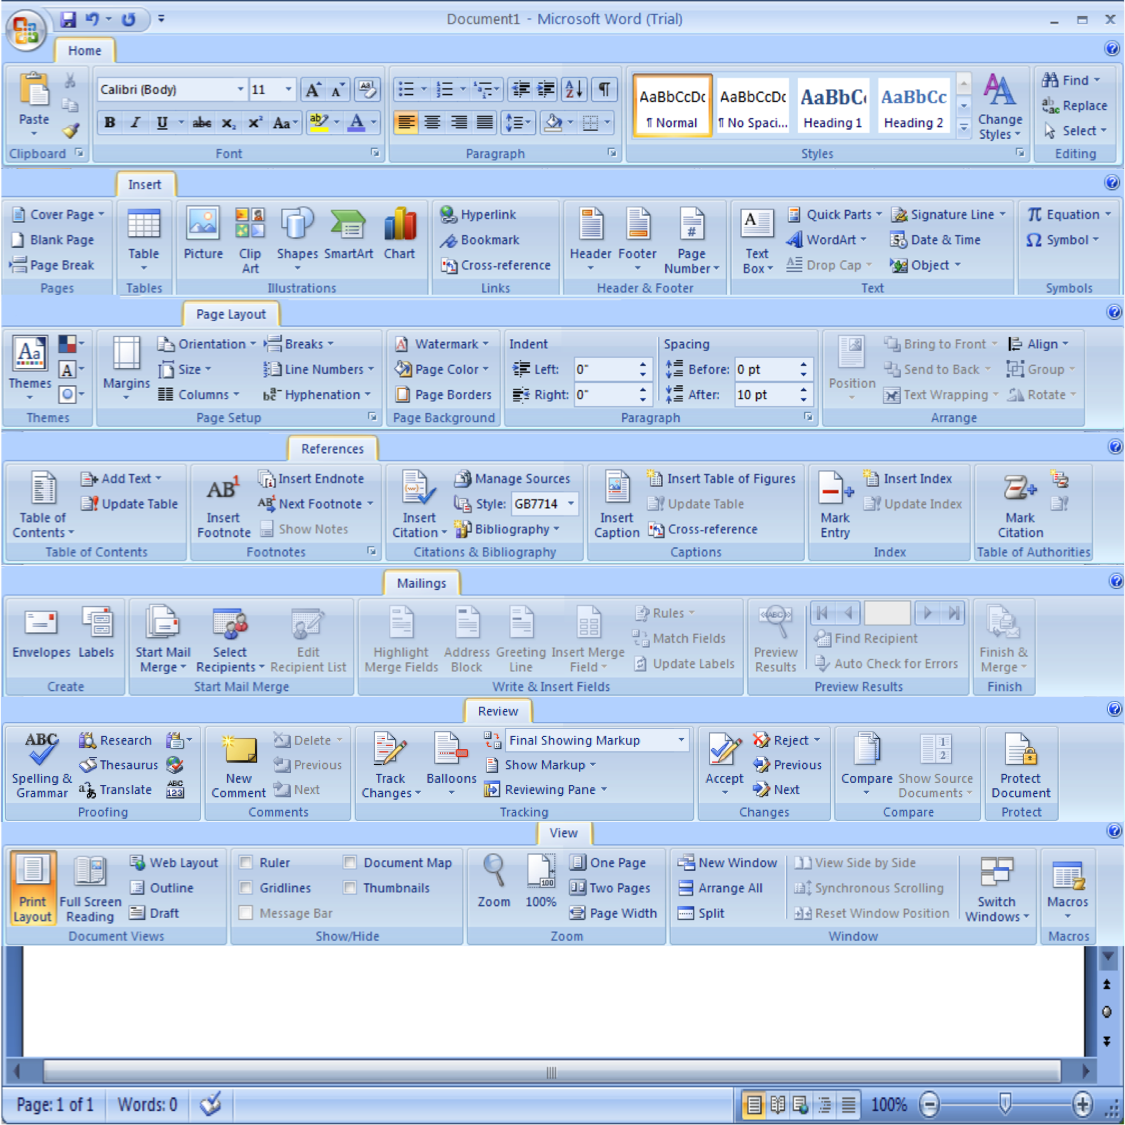
\includegraphics[width=80mm]{command_layout1}\\
  \caption{Our example CommandMap for Microsoft Word}
  \label{fig:ex_commandmap}
\end{figure}

%
%?	Independent variables: 
%o	Interface (layout of tabs)
%?	Dependent variables: 
%o	Selection time (seconds)
%o	Error rate (proportion)
%o	NASA-TLX measures [1,5] (mental demand, physical demand, temporal demand, hard work, frustration)
%o	Preference (Ribbon vs. CommandMaps)
%?	Control variables: 
%o	User's familiarity in MS Word - knowledgeable
%o	Resolution
%o	Computer specs
%o	Screen size
%o	
%?	Random variables: 
%o	Weather
%o	Temperature in the room
%o	Vision power of a participant
%o	Reaction rate of a participant
%o	Noise level
%o	Usual versions of MS Word that a participant uses
%
%?	Anything changed from what's described in the paper?
%o	Number and partitions of participants
%o	Computer specifications
%o	Screen size
%
%?	Any design choices that weren't clear in the paper that you had to figure out on your own?
%o	Methods of pointing (mouse, trackball, touchpad, joystick?) 
%o	Mouse acceleration
%o	Display of time 
%o	Presentation of instruction "as quickly and accurately as possible"
%o	Audible deep sound
%o	Definition of error rate 
%?	CMs inherently has a smaller number of TOTAL clicks if we include 'tab click' into 'total click'
%?	In Ribbon, tab click should not be included in TOTAL clicks 
%
%?	Threats to internal validity (Are observed results actually caused by the independent variables?); can we mitigate them?; how?
%o	If we were to perform this experiment throughout a week (not all on the same day), other external factors could threat internal validity
%o	How to mitigate: try to perform the experiments same time of days, same location (find an office, not a lounge), same lighting,  same computer, same mouse, and keyboard, same tasks, same training
%?	Threats to external validity (whether the effect we see can be generalized to the world outside the lab); can we mitigate them?; how?
%o	just doing the experiment, not other tasks (email, doc edits, etc) - cannot be mitigated at least for mimicing the study 2
%o	all location settings may be too constrained. overly artificial?
%o	1) chose a task that was a good match for the kinds of activities they had observed in the field. - most ppl like to work in a moderately quite environment. office is perfect!
%o	2) chose participants for the study that were as close as possible to those they studied in the field: good gender balance, ethnicity, age, etc
%o	3) assessed the similarity of the behaviors b/w the lab and the field. - nah 

\pagebreak

%\bibliographystyle{ieeepes}
%\bibliography{sarccdrefs}p

%%%%%%%%%%%%%%%%%%%%%%%%%%%%%%%%%%%%%%%%%%%%%%%%%%%%%%%%%%%%
%%%%%%%%%%%%%%%%%%%%%%%%%%%%%%%%%%%%%%%%%%%%%%%%%%%%%%%%%%%%

\end{document}
